\documentclass[12pt]{article}
\usepackage[margin=1in]{geometry} 
\usepackage{amsmath,amsthm,amssymb,amsfonts}
\usepackage{tikz,multirow,rotating}
 
\newcommand{\N}{\mathbb{N}}
\newcommand{\Z}{\mathbb{Z}}
 
\newenvironment{problem}[2][Problem]{\begin{trivlist}
\item[\hskip \labelsep {\bfseries #1}\hskip \labelsep {\bfseries #2.}]}{\end{trivlist}}
%If you want to title your bold things something different just make another thing exactly like this but replace "problem" with the name of the thing you want, like theorem or lemma or whatever
 
\begin{document}
 
%\renewcommand{\qedsymbol}{\filledbox}
%Good resources for looking up how to do stuff:
%Binary operators: http://www.access2science.com/latex/Binary.html
%General help: http://en.wikibooks.org/wiki/LaTeX/Mathematics
%Or just google stuff
 
\title{Discrete Math 2 HW 4}
\author{Ben Awad}
\maketitle
 
\begin{problem}{10.2.22}
\end{problem}

Yes. Group 1: [a, c] Group 2: [b, d, e]

\begin{problem}{10.2.24}
\end{problem}

Yes. Group 1: [f, c] Group 2: [a, b, e, d]

\begin{problem}{10.2.50}
\end{problem}

112

\begin{problem}{For the graph in 10.2.24, what is the subgraph induced by \{a, b, c, d\}?}
\end{problem}

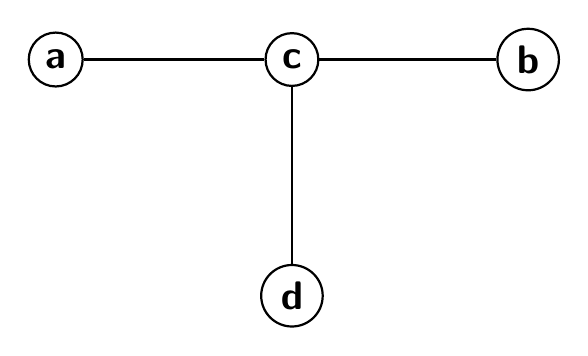
\begin{tikzpicture}[auto, node distance=3cm, every loop/.style={},
                    thick,main node/.style={circle,draw,font=\sffamily\Large\bfseries}]

  \node[main node] (a) {a};
  \node[main node] (c) [right of=a] {c};
  \node[main node] (b) [right of=c] {b};
  \node[main node] (d) [below of=c] {d};

  \path[every node/.style={font=\sffamily\small}]
  (a) edge node [right] {} (c)
  (c) edge node [right] {} (b)
  (c) edge node [below] {} (d)
  ;
\end{tikzpicture}

\begin{problem}{10.3.2}
\end{problem}

\begin{center}
    \begin{tabular}{ |c|c| } 
    \hline
    Vertex & Adjacent Vertices \\
    \hline
    a & b,d \\ 
    b & a,d,e \\ 
    c & d,e \\ 
    d & a,b,c \\ 
    e & b,c \\ 
    \hline
    \end{tabular}
\end{center}

\begin{problem}{10.3.4}
\end{problem}

\begin{center}
    \begin{tabular}{ |c|c| } 
    \hline
    Initial Vertex & Terminal Vertices \\
    \hline
    a & b,d \\ 
    b & a,c,d,e \\ 
    c & c,d \\ 
    d & a,e \\ 
    e & e,c \\ 
    \hline
    \end{tabular}
\end{center}

\begin{problem}{10.3.6}
\end{problem}

\begin{tabular}{|lr|l|l|l|l|l|l|l|l|l|} \cline{3-7}
\multicolumn{1}{l}{} & & A & B & C & D & E \\ \hline
%                           A   B   C   D   E  
& \multicolumn{1}{|r|}{A} & 0 & 1 & 0 & 1 & 0 \\ \cline{2-7}
& \multicolumn{1}{|r|}{B} & 1 & 0 & 0 & 1 & 1 \\ \cline{2-7}
& \multicolumn{1}{|r|}{C} & 0 & 0 & 0 & 1 & 1 \\ \cline{2-7}
& \multicolumn{1}{|r|}{D} & 1 & 1 & 1 & 0 & 0 \\ \cline{2-7}
& \multicolumn{1}{|r|}{E} & 0 & 1 & 1 & 0 & 0 \\ \hline
\end{tabular}

\begin{problem}{10.3.8}
\end{problem}

\begin{tabular}{|lr|l|l|l|l|l|l|l|l|l|} \cline{3-7}
\multicolumn{1}{l}{} && \multicolumn{5}{c|}{To} \\ \cline{3-7}
\multicolumn{1}{l}{} & & A & B & C & D & E \\ \hline
\multirow{5}{*}{\begin{sideways}From\end{sideways}}
%                           A   B   C   D   E  
& \multicolumn{1}{|r|}{A} & 0 & 1 & 0 & 1 & 0 \\ \cline{2-7}
& \multicolumn{1}{|r|}{B} & 1 & 0 & 1 & 1 & 1 \\ \cline{2-7}
& \multicolumn{1}{|r|}{C} & 0 & 1 & 1 & 0 & 0 \\ \cline{2-7}
& \multicolumn{1}{|r|}{D} & 1 & 0 & 0 & 0 & 1 \\ \cline{2-7}
& \multicolumn{1}{|r|}{E} & 0 & 0 & 1 & 0 & 1 \\ \hline
\end{tabular}

\begin{problem}{10.3.36}
\end{problem}

No: V has a vertex with degree 4 and U does not

\begin{problem}{10.3.38}
\end{problem}

Yes: $u_2 \rightarrow v_5$

$u_4 \rightarrow v_3$

$u_1 \rightarrow v_1$

$u_5 \rightarrow v_4$

$u_3 \rightarrow v_2$

\begin{problem}{10.3.40}
\end{problem}

No: V has a vertex with degree 4 and U does not

\begin{problem}{10.4.22}
\end{problem}

No because H has 2 symmetric rhombuses for paths which G does not have.

\begin{problem}{10.4.12}
\end{problem}

a. weak

b. strong

c. neither 

\begin{problem}{10.4.14}
\end{problem}

a. Component 1: a, b, e 

Component 2: d 

Component 3: c

b. Component 1: f

Component 2: c, e, d

Component 3: a

Component 4: b

c. Component 1: a, b, c, d, f, g, h, i

Component 2: e

\begin{problem}{10.4.50}
\end{problem}

a. $\lambda(G) = 2$, K(G) = 1, min deg = 2 so $K(G) < \lambda(G) \leq$ min deg

b. $\lambda(G) = 3$, K(G) = 1, min deg = 3 so $K(G) < \lambda(G) \leq$ min deg

c. $\lambda(G) = 2$, K(G) = 2, min deg = 3 so $K(G) \leq \lambda(G) <$ min deg

d. $\lambda(G) = 4$, K(G) = 4, min deg = 4 so $K(G) \leq \lambda(G) \leq$ min deg
\end{document}
